\documentclass[twoside,10pt]{article}
\usepackage{amsmath,amsfonts,amsthm,fullpage,amssymb}
%\usepackage{mymath}
\usepackage{algorithm,amsmath,amssymb}
\usepackage{algorithmic}
\usepackage{graphicx}
\usepackage{url}


\begin{document}


\title{
Richard Albright\\
ISYE 6740\\
Homework 5\\ 
Fall 2020\\}

%\date{Deadline: Feb. 13, Sat., 11:55pm}
\date{}
\maketitle



%As usual, please submit a report with sufficient explanation of your answers to each the questions, together with your code, in a zip folder.

%----------------------------------------------------------------------------------



\begin{enumerate}


\item{\bf SVM. } (45 points)

\begin{enumerate}
\item (5 points) Explain why can we set the margin $c = 1$ to derive the SVM formulation? 

$$\max_{w,b}{\frac{2c}{||w||}} \hspace{5 mm} s.t. \hspace{2 mm} y^i(w^T x^i + b) \geq c, \forall i$$

where the size of c is just scales the values of w and b.  Therefore we can just set c=1.  We can also drop the 2 to simplify the calculation and it becomes

$$\max_{w,b}{\frac{1}{||w||}} \hspace{5 mm} s.t. \hspace{2 mm} y^i(w^T x^i + b) \geq 1, \forall i$$

\item (10 points) Using Lagrangian dual formulation, show that the weight vector can be represented as
\[
w = \sum_{i=1}^n \alpha_i y_i x_i.
\]
where $\alpha_i \geq 0$ are the dual variables. What does this imply in terms of how to relate data to $w$?

The SVM solution can be expressed as the following convex optimization problem.

$$min_{w,b}\frac{1}{2}w^Tw  \hspace{5 mm} s.t. \hspace{2 mm} 1 - y^i (w^Tx^i + b) \leq 0, \forall i$$

$$ L(w,a,b) = \frac{1}{2}w^Tw + \sum^m_{i=1}{a_i(1 - y^i (w^Tx^i + b))}$$

$$ \frac{\partial{L}}{\partial{w}} = w - \sum^m_{i=1}{a_iy_ix_i} = 0 $$
$$ w = \sum^n_{i=1}{a_iy_ix_i}$$

This implies that the weight vector w linear combination of its datapoints and class labels.

\item (10 points) Explain why only the data points on the ``margin'' will contribute to the sum above, i.e., playing a role in defining $w$. 

$$min_{w,b}\frac{1}{2}w^Tw  \hspace{5 mm} s.t. \hspace{2 mm} 1 - y^i (w^Tx^i + b) \leq 0, \forall i$$

The KKT condition is

$$a_ig_i(w)=0 $$

$$a_i(1 - y^i (w^Tx^i + b)) = 0$$

where $$a_i = 0: \hspace{2 mm} 1 - y^i (w^Tx^i + b)) < 0$$
$$a_i > 0: \hspace{2 mm} 1 - y^i (w^Tx^i + b)) <= 0$$

only $a_i$ points that $>$ 0 lie on the margin and are the support vectors.

\item (20 points) Suppose we only have four training examples in two dimensions as shown in Fig. The positive samples at $x_1 = (0, 0)$, $x_2 = (2, 2)$ and negative samples at $x_3 = (h, 1)$ and $x_4 = (0, 3)$. 
%
\begin{center}
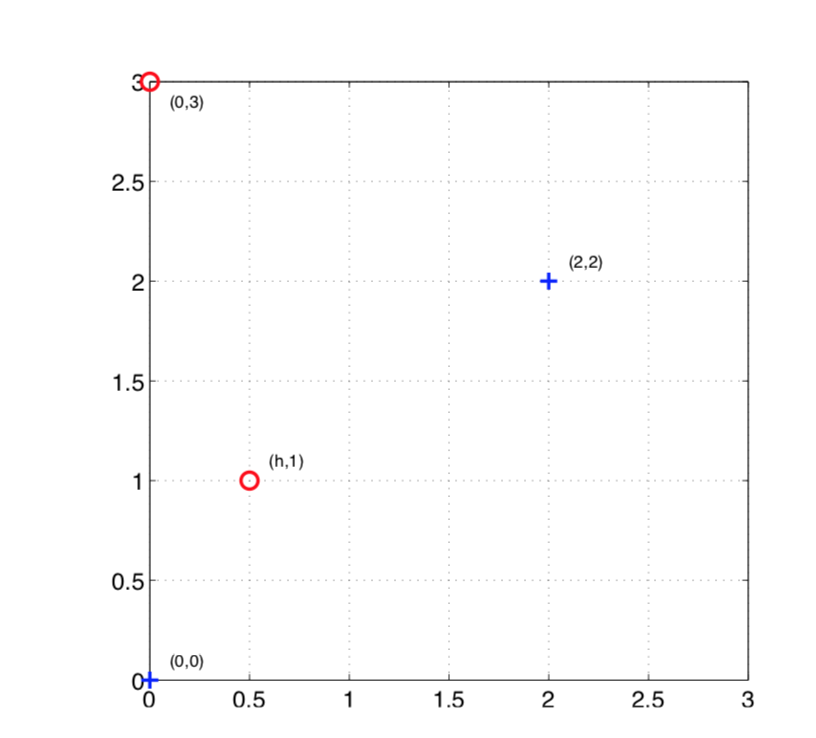
\includegraphics[width = 0.5\textwidth]{svm}
\end{center}

\begin{enumerate}
\item (10 points) For what range of parameter $h > 0$, the training points are still linearly separable?

\vspace{5 mm}
The training points are linearly separable for the range of $h > 0$ and $h < 1$, and at $h > 6$.
\vspace{5 mm}

\item (10 points) Does the orientation of the maximum margin decision boundary change as $h$ changes, when the points are separable?

\vspace{5 mm}
The orientation of the maximum decision boundary does not change as h changes when $h > 0$ and $h < 1$.  The decision boundary in this case has a positive slope and just shifts along the x axis as h changes. The orientation of the maximum decision boundary does change when $h > 6$. The slope is negative and gets more flat as $h$ increases.
\vspace{5 mm}
\end{enumerate}
\end{enumerate}



\item {\bf Multi-class classification for MNIST data set, comparison.} (55 points)

This question is to compare different classifiers and their performance for multi-class classifications on the complete MNIST dataset at \url{http://yann.lecun.com/exdb/mnist/}. You can find the data file \textsf{mnist\_10digits.mat} in the homework folder. The MNIST database of handwritten digits has a training set of 60,000 examples, and a test set of 10,000 examples. We will compare {\bf KNN, logistic regression, SVM, kernel SVM, and  neural networks}. We suggest to use \textsf{Scikit-learn}, which is a commonly-used and powerful \textsf{Python} library with various machine learning tools. But you can also use other similar libraries in other programming languages of your choice to perform the tasks. Below are some tips. 

\begin{itemize}

\item We suggest you to ``standardize'' the features before training the classifiers, by dividing the values of the features by 255 (thus map the range of the features from [0, 255] to [0, 1]).

\item You may adjust the number of neighbors $K$ used in KNN to have a reasonable result (you may use cross validation but it is not required; any reasonable tuning to get good result is acceptable).

\item You may use a neural networks function \textsf{sklearn.neural\_network} with \textsf{hidden\_layer\_sizes = (20, 10)}. 

%Tune the step size so you have reasonable results. You may use \textsf{svc} and tune the penalty term $C$ to get reasonable results. 

\item For kernel SVM, you may use  radial basis function kernel, and a heuristic called ``median trick'': choose the parameter of the kernel $K(x, x') = \exp\{-\|x-x'\|^2/(2\sigma^2)\}$. Choose the bandwidth as $\sigma=\sqrt{M/2}$ where $M =$ the median of $\{\|x^i-x^j\|^2, 1\leq i, j \leq m', i\neq j \}$ for pairs of training samples. Here you can randomly choose $m'=1000$ samples from training data to use for the ``median trick''\footnote{Garreau, Damien, Wittawat Jitkrittum, and Motonobu Kanagawa. "Large sample analysis of the median heuristic." arXiv preprint arXiv:1707.07269 (2017).}.

\item For KNN and SVM, you can randomly downsample the training data to size $m=5000$, to improve computation efficiency. 
\end{itemize}

Train the classifiers on training dataset and evaluate on the test dataset.

\begin{enumerate}

	\item (50 points) Report confusion matrix, precision, recall, and F-1 score for each of the classifiers. For precision, recall, and F-1 score of each classifier, we will  need to report these for each of the digits. So you can create a table for this. For this question, each of the 5 classifier, {\bf KNN, logistic regression, SVM, kernel SVM, and  neural networks}, accounts for 10 points.
	
	\vspace{5 mm}
	
	An area under the curve analysis was performed to find the optimal $k$ value for knn. Based on the chart below, I chose $k = 6$.
	
	\begin{center}
	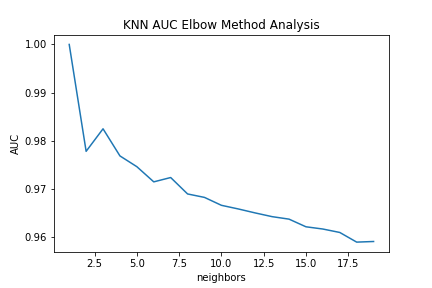
\includegraphics[width = 0.4\textwidth]{knn_auc}
	\end{center}
	
	\vspace{80 mm}
	
	Using the tips provided for question 2, below are the results for the classifiers KNN, Logistic Regression, Linear SVM, Kernel SVM, and Neural Network (Please excuse the word cutoffs for macro avg and weighted avg, I couldn't figure out how to fix it).
	
	\begin{center}
	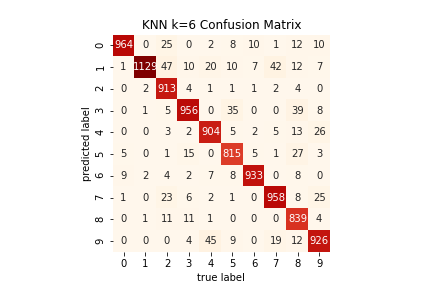
\includegraphics[width = 0.44\textwidth]{knn}
	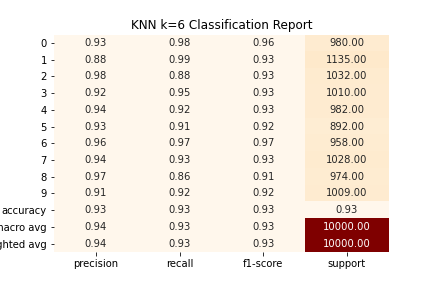
\includegraphics[width = 0.44\textwidth]{knn_class}
	\end{center}

	\begin{center}
	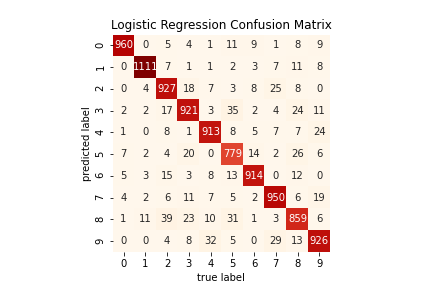
\includegraphics[width = 0.44\textwidth]{logistic}
	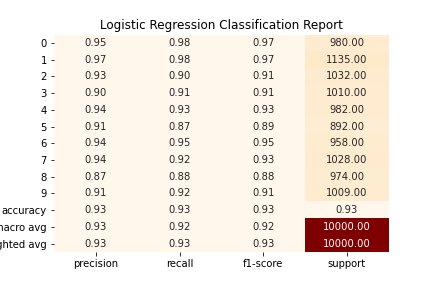
\includegraphics[width = 0.44\textwidth]{logistic_class}
	\end{center}
	
	\begin{center}
	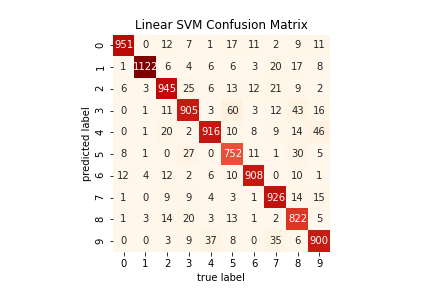
\includegraphics[width = 0.44\textwidth]{linearsvm}
	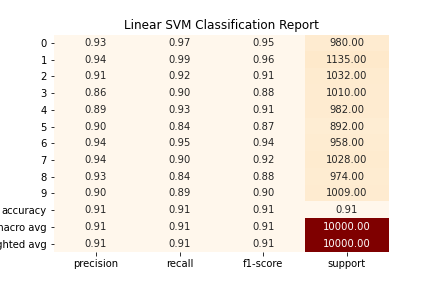
\includegraphics[width = 0.44\textwidth]{linearsvm_class}
	\end{center}
	
	\begin{center}
	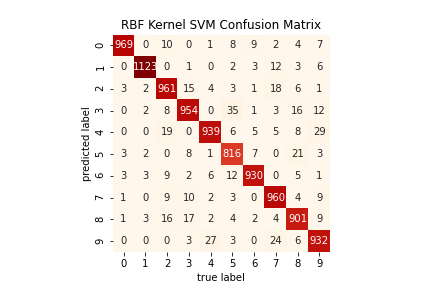
\includegraphics[width = 0.44\textwidth]{kernelsvm}
	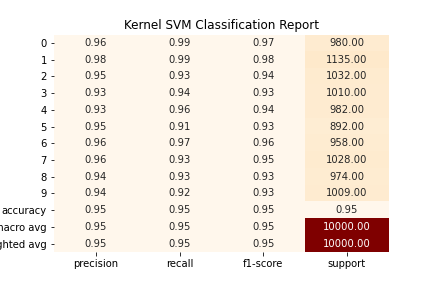
\includegraphics[width = 0.44\textwidth]{kernelsvm_class}
	\end{center}
	
	\begin{center}
	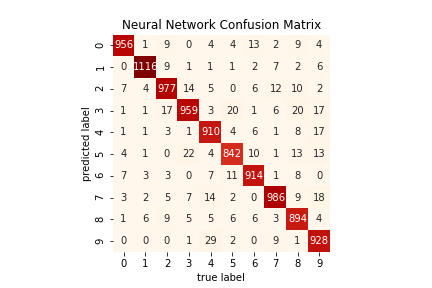
\includegraphics[width = 0.44\textwidth]{neural}
	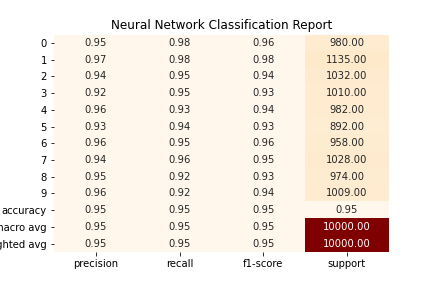
\includegraphics[width = 0.44\textwidth]{neural_class}
	\end{center}
	

	
	\item (5 points) Comment on the performance of the classifier and give your explanation why some of them perform better than the others.	
	
\vspace{5 mm}

All classifiers resulted in accuracies of over $90\%$. Linear SVM performed the worst, while RBF Kernel SVM and Neural Network performed the best.  KNN had the hardest time classifying 1.  My guess is that is harder to pick the nearest neighbors accurately beause there is less variation on the horizontal axis, leaving mostly the vertical axis to determine the nearest neighbors.  Logistic regression had the hardest time classifying 8.  Since the sigmoid function's 1st derivative is symmetric, it might have a harder time determinine 8 from other numbers since it is mostly symmetric along its vertical axis. Linear SVM performs generally worse, likely because the images are not strictly linearly separable.  RBF Kernel SVM shows a marked improvement over Linear SVM. The gamma parameter was adjusted using the median trick.  The classification rates for 3 and 4 were the lowest for the RBF Kernel SVM, while still maintaining an accuracy rate of over $93\%$.  The number 3 was most oftenly misclassified as 8, while 4 was most oftenly misclassified as 9. Nueral Network classification had the worst performance classifying both 3 and 5. They both were most often misclassified as each other.  I would have expected Neural Network to perform the best, because this algorithm is best candidate for classifying images.  
\end{enumerate}

\vspace{5 mm}

\item {\bf Neural networks.} (Bonus: 10 points)

\begin{enumerate}
\item (2 points)
Consider a neural networks for a binary classification using sigmoid function for each unit. If the network has no hidden layer, explain why the model is equivalent to logistic regression. 

\vspace{5 mm}

A neural network consists of an input layer, a hidden layer, and an output layer.  The input layer consists of the independent variables + the bias term.  The hidden layer consists of nonlinear transformation functions that bound the continuous input variables to a value between 0 and 1.  Each nonlinear function is given a weight between 0 and 1 where the sum of weights = 1.  The output layer consists of a sigmoid function to convert the output of the last layer into a probability of belonging to a given class.  By removing the hidden layer, we end up taking the input layer as inputs into the sigmoid function, which is the logistic regression model.

\vspace{5 mm}

\item (8 points) 
Consider a simple two-layer network in the lecture slides. Given $m$ training data $(x^i, y^i)$, $i = 1, \ldots, m$, the cost function used to training the neural networks
\[
\ell(w, \alpha, \beta) = \sum_{i=1}^m (y^i - \sigma(w^T z^i))^2
\]
where $\sigma (x) = 1/(1+e^{-x})$ is the sigmoid function, $z^i$ is a two-dimensional vector such that  $z_1^i = \sigma(\alpha^T x^i)$, and $z_2^i = \sigma(\beta^T x^i)$. Show the that the gradient is given by
\[
\frac{\partial \ell(w, \alpha, \beta) }{\partial w}
= - \sum_{i=1}^m 2(y^i - \sigma(u^i))\sigma(u^i)(1-\sigma(u^i)) z^i,
\]
where $u^i = w^T z^i$. Also find the gradient of $\ell(w, \alpha, \beta)$ with respect to $\alpha$ and $\beta$ and write down their expression.

\vspace{5 mm}
The gradient of $\ell(w, \alpha, \beta)$ with respect to $w$

$$\frac{\partial \ell(w, \alpha, \beta) }{\partial w} = 
 \frac{\partial{\sum_{i=1}^m (y^i - \sigma(w^T z^i))^2}}{\partial{w}}$$
 
$$=\sum_{i=1}^m{\frac{\partial{((y^i - \sigma(w^T z^i))^2)}}{\partial{w}}}$$

$$=\sum_{i=1}^m{ \frac{\partial{((y^i - \sigma(w^T z^i))^2)}}{\partial{(y^i - \sigma(w^T z^i))}} \frac{\partial{(y^i - \sigma(w^T z^i))}}{\partial{w}} }$$

$$=\sum_{i=1}^m{2(y^i - \sigma(w^T z^i))(\frac{\partial{y^i}}{\partial{w}}   -   \frac{\partial{\sigma(w^T z^i)}}{\partial{w}})}$$

$$=- \sum_{i=1}^m{2(y^i - \sigma(w^T z^i)) \frac{\partial{\sigma(w^T z^i)}}{\partial{w^T z^i}} \frac{\partial{w^T z^i}}{\partial{w}}} $$

$$= - \sum_{i=1}^m{2(y^i - \sigma(w^T z^i)) \frac{\partial{\sigma(w^T z^i)}}{\partial{w^T z^i}} z^i}$$

$$=- \sum_{i=1}^m{2(y^i - \sigma(u^i)) \frac{\partial{\sigma(u^i)}}{\partial{u^i}} z^i} $$

$$=- \sum_{i=1}^m{2(y^i - \sigma(u^i)) \frac{\partial{(1/(1+e^{-u^i}))}}{\partial{u^i}} z^i} $$

$$=- \sum_{i=1}^m{2(y^i - \sigma(u^i)) z^i \frac{(\partial{1}/\partial{u^i})(1+e^{-u^i}) -  \partial{(1+e^{-u^i})} / \partial{u^i}} {(1+e^{-u^i})^2}} $$

$$=- \sum_{i=1}^m{2(y^i - \sigma(u^i)) z^i \frac{e^{-u^i}} {(1+e^{-u^i})^2}}$$

$$=- \sum_{i=1}^m{2(y^i - \sigma(u^i)) \frac{1}{1+e^{-u^i}} (1 - \frac{1}{1+e^{-u^i}}) z^i }$$

$$=- \sum_{i=1}^m 2(y^i - \sigma(u^i))\sigma(u^i)(1-\sigma(u^i)) z^i$$

\vspace{10 mm}
The gradient of $\ell(w, \alpha, \beta)$ with respect to $\alpha$.

\vspace{2 mm}

Using the chain rule.


$$\frac{\partial \ell(w, \alpha, \beta) }{\partial \alpha} = \frac{\partial \ell(w, \alpha, \beta) }{\partial z_1^i} \frac{\partial z_1^i}{\partial \alpha}$$


$$\frac{\partial \ell(w, \alpha, \beta) }{\partial z_1^i} = \sum_{i=1}^m {\frac{\partial ((y^i - \sigma(w^T z^i_1))^2) }{\partial z_1^i}}$$

$$=- \sum_{i=1}^m {2(y^i - \sigma(u^i))\sigma(u^i)(1-\sigma(u^i)) w_1}$$

Therefore

$$\frac{\partial \ell(w, \alpha, \beta) }{\partial \alpha} = \frac{\partial \ell(w, \alpha, \beta) }{\partial z_1^i} \frac{\partial z_1^i}{\partial \alpha} $$

$$=\sum_{i=1}^m {\frac{\partial ((y^i - \sigma(w^T z^i_1))^2) }{\partial z_1^i} \frac{\partial (\sigma(\alpha^T x^i))}{\partial \alpha}}$$

$$ =- \sum_{i=1}^m {2(y^i - \sigma(u^i))\sigma(u^i)(1-\sigma(u^i)) w_1 \frac{\partial (\sigma(\alpha^T x^i))}{\partial \alpha}}$$

$$=- \sum_{i=1}^m {2(y^i - \sigma(u^i))\sigma(u^i)(1-\sigma(u^i)) w_1 \frac{\partial (1/(1+e^{-\alpha^Tx^i}))}{\partial \alpha}} $$

$$=- \sum_{i=1}^m {2(y^i - \sigma(u^i))\sigma(u^i)(1-\sigma(u^i)) w_1 \frac{(\partial{1}/\partial{\alpha})(1+e^{-\alpha^Tx^i}) -  \partial{(1+e^{-\alpha^Tx^i})} / \partial{\alpha}} {(1+e^{-\alpha^Tx^i})^2}}$$

$$=- \sum_{i=1}^m {2(y^i - \sigma(u^i))\sigma(u^i)(1-\sigma(u^i)) w_1 \frac{ e^{-\alpha^Tx^i}} {(1+e^{-\alpha^Tx^i})^2}x_i}$$

$$=- \sum_{i=1}^m {2(y^i - \sigma(u^i))\sigma(u^i)(1-\sigma(u^i)) w_1 \frac{1}{1+e^{-\alpha^Tx^i}} (1 - \frac{1}{1+e^{-\alpha^Tx^i}})x_i}$$

$$= - \sum_{i=1}^m {2(y^i - \sigma(u^i))\sigma(u^i)(1-\sigma(u^i)) w_1 \sigma(\alpha^T x^i) (1 - \sigma(\alpha^T x^i))x_i}$$

\vspace{2 mm}

The gradient of $\ell(w, \alpha, \beta)$ with respect to $\beta$.

\vspace{2 mm}

Performing a similar calculation for $\beta$ in the above derivation we get:

$$\frac{\partial \ell(w, \alpha, \beta) }{\partial \beta} = 
- \sum_{i=1}^m {2(y^i - \sigma(u^i))\sigma(u^i)(1-\sigma(u^i)) w_1 \sigma(\beta^T x^i) (1 - \sigma(\beta^T x^i))x_i} $$
\vspace{5 mm}
\end{enumerate}
\end{enumerate}
\end{document}
